\Chapter{Problem układania planu lekcji i algorytm jego rozwiązania}\label{chapter:algorytm}
    Opis struktury rozdziału.
    % Chociaż czyste podejście MIP prowadzi do teoretycznie optymalnych rozwiązań, w praktyce jego zastosowanie do pełnego problemu jest niemożliwe.
    % Złożoność obliczeniowa i pamięciowa przekracza możliwości przeciętnych komputerów, co uniemożliwia efektywny rozwój takiego rozwiązania.
    % Ponadto takie rozwiązanie jest też trudne do zaprogramowania ze względu na bloki lekcyjne.

    % Zaprezentowane podejście hybrydowe pozwala pokonać problem złożoności obliczeniowej, oferując praktyczny kompromis między optymalnością a czasem obliczeń.

    \section{Sformułowanie problemu optymalizacyjnego}
        Na potrzeby pracy warto ujednolicić terminologię, z uwagi na to, że w języku potocznym niektóre z tych terminów są używane zamiennie:
        \begin{itemize}
            \item \textbf{Klasa}: Grupa uczniów; przykładowo ,,IIA'', ,,IVC'', \dots
            Ze względu na angielską nazwę \textit{class}, która koliduje ze składnią języków programowania, w kodzie często odnoszę się do klas jako \verb|student_group|.
            \item \textbf{Sala}: Miejsce, w którym prowadzone są zajęcia; przykładowo ,,Sala Gimnastyczna 1'', ,,2'', \dots
            \item \textbf{Przedmiot}: Temat zajęć prowadzonych przez nauczyciela; przykładowo ,,Wychowanie Fizyczne'', ,,Matematyka'', \dots
            \item \textbf{Lekcja}: Zajęcia prowadzone przez jednego nauczyciela, w jednej sali, z jedną lub więcej klas, które są na temat jednego przedmiotu.
            \item \textbf{Slot czasowy}: Czas w którym odbywa się lekcja; przykładowo slot zerowy może odbywać się od 7:00 do 7:45.
            \item \textbf{Blok lekcyjny}: Grupa dwóch lub więcej lekcji, które odbywają się w tym samym slocie czasowym.
            Mogą one dotyczyć jednej klasy oraz wielu nauczycieli, jednego nauczyciela i wielu klas, lub też wielu klas i wielu nauczycieli.
            \item \textbf{Okienko}: Przerwa między dwoma lekcjami klasy lub nauczyciela. Występuje gdy zajęcia nie są przeprowadzane bezpośrednio po sobie.
        \end{itemize}

        Problem optymalizacyjny w tej pracy polega na przypisaniu lekcji do odpowiednich slotów czasowych i sal przy jednoczesnym spełnieniu wymagań.
        W rzeczywistości sformułowanie takiego zadania i wyznaczenie jego rozwiązania stanowi duże wyzwanie.
        Istnieją ograniczenia, które są różne dla każdej klasy, co utrudnia formułowanie problemu --- wiele lekcji jest realizowanych w blokach, które są definiowane każdy z osobna.
        Przez te wyjątki nie jest możliwym wykorzystanie prostych algorytmów.
        Nie jest także możliwym rozwiązanie jednego wielkiego problemu programowania całkowitoliczbowego w sensownym czasie przy użyciu komputera z przeciętną specyfikacją.
        
        \subsection{Dane i szukane}
            \subsubsection{Słownik podstawowych oznaczeń}\label{slownik_oznaczen}
                \begin{itemize}
                    \item $\mathcal{C}$ --- zbiór klas
                    \item $\mathcal{T}$ --- zbiór nauczycieli  
                    \item $\mathcal{S}$ --- zbiór przedmiotów
                    \item $\mathcal{R}$ --- zbiór sal
                    \item $\vec{R_{i}}$ --- zbiór przedmiotów obsługiwanych przez $i$-tą salę
                    % \item $\mathcal{W}$ --- zbiór wymagań głównych
                    % \item $\mathcal{L}$ --- zbiór bloków lekcyjnych
                    % \item $\mathcal{B}$ --- zbiór bloków przedmiotów
                    \item $H$ --- liczba slotów czasowych w dniu
                    % \item $V$ --- wektor godzin bloków
                    % \item $A$ --- macierz dostępności nauczycieli
                    % \item $S$ --- macierz przydziału do dni, kodowanie osobnika
                    % \item $\mathfrak{P}$ --- wielkość populacji w algorytmie ewolucyjnym !DO PRZENIESIENIA!
                \end{itemize}

            \subsubsection{Wymagania główne}
                Warto zacząć od przedstawienia sposobu reprezentacji zmiennych zaczynając od wymagań głównych.
                Ilość godzin tygodniowo odbytych przez klasę z danym nauczycielem w ramach danego przedmiotu jest z góry ustalona.
                Aby łatwiej zrozumieć na czym polegają takie przypisania warto spojrzeć na dotychczasowy sposób przypisywania ilości godzin nauczycieli do klas w liceum, które dostarczyło dane na potrzeby tej pracy.
            
                \begin{figure}[H]
                    \centering
                    \includegraphics[width=0.9\textwidth]{images/excel_wymagania.png}
                    \caption{Zrzut ekranu z arkusza kalkulacyjnego przedstawiąjący przypisanie godzinowe nauczycieli dla każdej klasy.}\label{fig:excel_wymagania}
                \end{figure}
                Każdy nauczyciel jest przypisany do prowadzonych przez niego przedmiotów. 
                Następnie w odpowiednim wierszu nauczyciela, pod odpowiednim przedmiotem, w kolumnie każdej klasy definiowana jest ilość godzin, która będzie poświęcona na prowadzenie tego przedmiotu.

                Zbiór takich wymagań $\mathcal{W}$ definiuje się następująco:
                \begin{equation}\label{eq:wymaganie_glowne}
                    w_i \triangleq \left(t_{w_i}, c_{w_i}, s_{w_i}, g_{w_i}\right) \in \mathcal{W}, \quad \forall i \in \left\{1, 2, \dots, \left|\mathcal{W}\right|\right\}: \begin{cases} t_{w_i} &\in \mathcal{T}\\c_{w_i} &\in \mathcal{C}\\s_{w_i} &\in \mathcal{S}\\g_{w_i} &\in \mathbb{N}^+ \end{cases}
                \end{equation}
                gdzie $g_{w_i}$ to liczba wymaganych tygodniowo godzin przedmiotu $s_{w_i}$ przeprowadzonego przez nauczyciela $t_{w_i}$ dla klasy $c_{w_i}$.

            \subsubsection{Dostępnośc nauczycieli}
                Każdy nauczyciel ma też zdefiniowaną dostępność, która jest reprezentowana przez macierz $A$ o wymiarach $\left|\mathcal{T}\right|$ na $5$, gdzie $\left|\mathcal{T}\right|$ to liczba wszystkich nauczycieli.
                Macierz jest zero-jedynkowa, gdzie 1 oznacza, że $t$-ty nauczyciel jest dostępny $d$-tego dnia tygodnia, a 0 że jest niedostepny.
                \[ A = \begin{bmatrix}
                    a_{1,1} & a_{1,2} & \cdots & a_{1,5} \\
                    a_{2,1} & a_{2,2} & \cdots & a_{2,5} \\
                    \vdots & \vdots & \ddots  & \vdots  \\
                    a_{\left|\mathcal{T}\right|,1} & a_{\left|\mathcal{T}\right|,2} & \cdots & a_{\left|\mathcal{T}\right|,5} \\
                \end{bmatrix}, \quad \forall t \in \mathcal{T}, d \in \left\{1, 2, 3, 4, 5\right\}: a_{t, d} \in \left\{0, 1\right\} \]
            
            \subsubsection{Bloki przedmiotów}\label{subject_blocks}
                W celu tworzenia bloków lekcyjnych mamy także dostęp do zbioru bloków przedmiotów $\mathcal{B}$:
                \[
                    b_i \triangleq \left(\vec{S_{b_i}},\vec{C_{b_i}}, \vec{G_{b_i}}, \verb|is_aggregating|_{b_i}, \verb|max_weekly|_{b_i}\right) \in \mathcal{B}
                \]
                \[ \forall i \in \left\{1, 2, \dots, \left|\mathcal{B}\right|\right\}: \begin{cases}
                    \vec{S_{b_i}} &\subset \mathcal{S} \\
                    \vec{C_{b_i}} &\subseteq  \mathcal{C} \\
                    \vec{G_{b_i}} &\in \mathbb{N}^{\left|\vec{S_b}\right|} \\
                    \verb|is_aggregating|_{b_i} &\in \left\{0, 1\right\} \\
                    \verb|max_weekly|_{b_i} & \in \mathbb{N}
                \end{cases} \]
                gdzie
                \begin{itemize}
                    \item $\vec{S_{b_i}}$ to podzbiór wszystkich przedmitów, których dotyczy blok $b_i$,
                    \item $\vec{C_{b_i}}$ to podzbiór wszystkich klas, których dotyczy blok $b_i$,
                    \item $\vec{G_{b_i}}$ to wektor oczekiwanej liczby przedmiotów w bloku.
                    \item $\verb|is_aggregating|$ to wartość binarna informująca o tym czy blok jest \textit{agregujący}, to znaczy czy służy w celu łączenia innych bloków w jeszcze większe bloki.
                    \item $\verb|max_weekly|$ to liczba naturalna która informuje o maksymalnej liczbie bloków. Jeśli $\verb|max_weekly|=0$ to oznacza to, że liczba bloków jest nielimitowana.
                \end{itemize}
                Przykładowy blok przedmiotów:
                \begin{itemize}
                    \item $\vec{S_b} = \text{(język angielski, informatyka)}$,
                    \item $\vec{C_b} = \text{(IA, IB, IC)}$,
                    \item $\vec{G_b} = \left(1, 1\right)$,
                    \item $\verb|is_aggregating| = 0$,
                    \item $\verb|max_weekly| = 0$.
                \end{itemize}
                lub:
                \begin{itemize}
                    \item $\vec{S_b} = \text{(język angielski)}$,
                    \item $\vec{C_b} = \mathcal{C}$
                    \item $\vec{G_b} = \left(2\right)$,
                    \item $\verb|is_aggregating| = 0$,
                    \item $\verb|max_weekly| = 0$.
                \end{itemize}

            \subsubsection{Bloki lekcyjne}
                Blok lekcyjny $L$ jest zbiorem wymagań głównych, które mogą być realizowane w ramach jednej bądź wielu lekcji jednocześnie.

                Zbiór takich bloków lekcyjnych $\mathcal{L}$ definiujemy następująco:
                \[ \mathcal{L} = \left\{L_1, L_2, \dots, L_{\left|\mathcal{L}\right|}\right\}, \quad \forall i \in \left\{1, 2, \dots, \left|\mathcal{L}\right|\right\}: L_i \subset \mathcal{W} \]

                Przykładowe interpretacje bloków lekcyjnych:
                \begin{itemize}
                    \item 3 godziny języka angielskiego z klasą IA prowadzone przez nauczyciela angielskiego 1,
                    \item 3 godziny języka angielskiego z klasą IA prowadzone przez nauczyciela angielskiego 2,
                \end{itemize}
                w przypadku różnych przedmiotów:
                \begin{itemize}
                    \item 3 godziny języka angielskiego z klasą IA prowadzone przez nauczyciela angielskiego 1,
                    \item 2 godziny informatyki z klasą IA prowadzone przez nauczyciela informatyki 1,
                \end{itemize}
                lub dla różnych klas:
                \begin{itemize}
                    \item 1 godzina języka francuskiego z klasą IA prowadzona przez nauczyciela francuskiego 1,
                    \item 1 godzina języka francuskiego z klasą IB prowadzona przez nauczyciela francuskiego 1,
                \end{itemize}

            \subsubsection{Szukane}
                Oczekiwanym rezultatem działania algorytmu powinien być zbior przypisań $\mathcal{Z}$. Każde takie przypisanie powinno mieć 6 wartości:\label{fragment:przypisania}
                \[ z_i \triangleq \left(d_{z_i},h_{z_i},c_{z_i},t_{z_i},s_{z_i},r_{z_i}\right) \in \mathcal{Z}, \quad \forall i \in \left\{0, 1, \dots, \left|\mathcal{Z}_d\right|\right\}: \begin{cases} d_{z_i} &\in \left\{1, 2, 3, 4, 5\right\} \\h_{z_i} &\in \left\{0, 1, \dots, H\right\}\\ c_{z_i} &\in \mathcal{C}\\ t_{z_i} &\in \mathcal{T}\\s_{z_i} &\in \mathcal{S}\\r_{z_i} &\in \mathcal{R} \end{cases} \]
                Przykładowe interpretacje takich przypisań:
                \begin{itemize}
                    \item Poniedziałek, Slot czasowy 0, IA,\ \ nauczyciel francuskiego 1, język francuski, Sala nr 1
                    \item Poniedziałek, Slot czasowy 0, IIA, nauczyciel francuskiego 1, język francuski, Sala nr 1
                    \item[$\vdots$]
                    \item Piątek, Slot czasowy 10, IVC, nauczyciel fizyki 2, fizyka, Sala nr 15
                \end{itemize}
                W przypadku lekcji, która obejmują więcej klas niż jedna, należy stworzyć przypisanie dla każdej klasy osobno.
            
        \subsection{Ograniczenia}\label{subsection:ograniczenia}
            Wcześniej wspomniane ograniczenia można podzielić na 4 kategorie:

            \subsubsection{Ograniczenia fizyczne}
                \begin{itemize}
                    \item Żaden nauczyciel nie może być w 2 miejscach na raz.
                    \begin{align*}
                        \forall i, j \in \left\{1, 2, \dots, \left|\mathcal{Z}\right|\right\}:\\
                        t_{z_i} = t_{z_j} \implies \left[i = j \lor d_{z_i} \neq d_{z_j} \lor h_{z_i} \neq h_{z_j} \lor \left(d_{z_i} = d_{z_j} \land h_{z_i} = h_{z_j} \land r_{z_i} = r_{z_j}\right)\right]
                    \end{align*}
                    \item Nauczyciel musi być dostępny.
                    \[ \forall i \in \left\{1, 2, \dots, \left|\mathcal{Z}\right|\right\}: a_{t_{z_i},d_{z_i}} = 1 \]
                    \item Żaden uczeń nie może być w 2 miejscach na raz.
                    \begin{align*}
                        \forall i, j \in \left\{1, 2, \dots, \left|\mathcal{Z}\right|\right\}, \exists k \in \left\{1, 2, \dots \left|\mathcal{B}\right|\right\}:\\
                        \left(d_{z_i} = d_{z_j} \land h_{z_i} = h_{z_j} \land c_{z_i} = c_{z_j} \land i \neq j \right) \implies c_{z_i} \in \vec{C_{b_k}} \land s_{z_i},s_{z_j} \in \vec{S_{b_k}}
                    \end{align*}
                    \item W żadnej sali nie mogą odbywać się 2 lekcje na raz.
                    \begin{align*}
                        \forall i, j \in \left\{1, 2, \dots, \left|\mathcal{Z}\right|\right\}, \exists k \in \left\{1, 2, \dots \left|\mathcal{B}\right|\right\}:\\
                        \left(d_{z_i} = d_{z_j} \land h_{z_i} = h_{z_j} \land r_{z_i} = r_{z_j} \land i \neq j \right) \implies s_{z_i} = s_{z_j} \land s_{z_i}, s_{z_j} \in \vec{S_{b_k}}
                    \end{align*}
                \end{itemize}
                
                \begin{samepage}
                    \textbf{Ograniczenia prawne}~\cite{karta_nauczyciela, prawo_oswiatowe, obwieszczenie}
                        \begin{itemize}
                            \item Uczeń nie może mieć więcej niż 2 godzin lekcyjnych tego samego przedmiotu dziennie.
                            \[ \forall d \in \left\{1, 2, 3, 4, 5\right\}, c \in \mathcal{C}, s \in \mathcal{S}: \left|\left\{z \in \mathcal{Z}: d_z = d \land c_z = c \land s_z = s\right\}\right| \leq 2 \]
                            \item Jeśli danego dnia mają zostać przeprowadzone 2 godziny jednego przedmiotu, to uczeń musi je mieć bezpośrednio po sobie.
                            \begin{align*}
                                \forall i, j \in \left\{1, 2, \dots, \left|\mathcal{Z}\right|\right\}, c \in \mathcal{C}, s \in \mathcal{S}:\\
                                \left(d_{z_i} = d_{z_j} \land c_{z_i} = c_{z_j} \land s_{z_i} = s_{z_j} \land i \neq j \right) \implies \left|h_{z_i} - h_{z_j}\right| = 1
                            \end{align*}
                        \end{itemize}
                \end{samepage}

            \subsubsection{Ograniczenia jakościowe}
                \begin{itemize}
                    \item Brak okienek dla uczniów. Nie istnieje taka para przypisań, dla których różnica między slotami czasowymi jest większa niż suma wszystkich lekcji danego dnia.
                    \begin{align*}
                        \nexists i, j \in \left\{1, 2, \dots, \left|\mathcal{Z}\right|\right\}, c \in \mathcal{C}:\\
                        d_{z_i} = d_{z_j} \land c_{z_i} = c_{z_j} \land \left|h_{z_i} - h_{z_j}\right| > \left|\left\{z_k: d_{z_k} = d_{z_i} \land c_{z_i}\right\}\right|
                    \end{align*}
                    \item Odpowiednie przypisanie sal. Lekcje wychowania fizycznego muszą odbyć się w przeznaczonych do tego salach, podobnie lekcji informatyki itd.
                    \[ \forall z \in \mathcal{Z}: s_z \in \vec{R_{r_z}} \]
                    \item Dla bloków lekcyjnych, które odbywają się 3 razy w tygodniu konieczne jest stworzenie jednego bloku dwugodzinnego.
                    \begin{align*}
                        \forall w \in \mathcal{W}, \exists d \in \left\{1, 2, 3, 4, 5\right\}: \\ 
                        g_w = 3 \implies \left|\left\{z \in \mathcal{Z}: c_w = c_z \land s_w = s_z \land t_w = t_z \land d_z = d \right\}\right| = 2
                    \end{align*}
                \end{itemize}

            \subsubsection{Ograniczenie główne}
                Zgodnie z definicją przyjętą w~\ref{eq:wymaganie_glowne} tygodniowa liczba godzin każdego przedmiotu musi być równa tej ustalonej w zbiorze wymagań:
                \[ \forall w \in \mathcal{W}: \left|\left\{z \in \mathcal{Z}: c_w = c_z \land t_w = t_z \land s_w = s_z\right\}\right| = g_w \]

            \subsubsection{Hierarchiczna dekompozycja problemu}
                Podczas gdy w pracy~\cite{rappos2022mixed} dekompozycja dotyczy głównie warstw ograniczeń, w moim rozwiązaniu wprowadziłem dekompozycję całego problemu:

            Każdy poziom rozwiązuje inny problem i wykorzystuje odpowiednie do tego celu algorytmy.

            \subsubsection{Kombinacja metod optymalizacyjnych}
                W odróżnieniu od pracy źródłowej, która wykorzystuje wyłącznie solver MIP z heurystykami, w moim podejściu zastosowałem wiele technik:
                \begin{itemize}
                    \item \textbf{Algorytm zachłanny} --- dla problemów konstrukcyjnych (tworzenie bloków)
                    \item \textbf{Algorytm ewolucyjny} --- dla dyskretnego przydziału bloków do dni
                    \item \textbf{Solver CP} --- dla problemów szeregowania
                \end{itemize}

            \subsubsection{Redukcja złożoności obliczeniowej}
                Pełny problem harmonogramowania wymagałby liczby zmiennych decyzyjnych proporcjonalnych do:
                \[ |\mathcal{T}| \times |\mathcal{C}| \times |\mathcal{S}| \times 5 \times H \times |\mathcal{R}| \]milionów
                co dla typowej szkoły daje miliony potencjalnych zmiennych.
            
                W podejściu dekompozycyjnym:
                \begin{itemize}
                    \item \textbf{Etap 1}: Operuje na $|\mathcal{W}|$ wymaganiach
                    \item \textbf{Etap 2}: Operuje na $5 \times |\mathcal{L}|$ zmiennych
                    \item \textbf{Etap 3}: Rozwiązuje 5 niezależnych podproblemów o rozmiarze 20\% oryginalnego problemu
                \end{itemize}

                Każdy etap można modyfikować lub wymieniać niezależnie. Jest to ważna zaleta podczas rozwijania oprogramowania.
                W szczególności jeśli takie oprogramowanie może być w przyszłości rozwijane przez więcej niż jednego dewelopera.

\section{Poprzednie podejścia}
    Aby w pełni zrozumieć mój wybór narzędzi warto szybko przetoczyć historię moich poprzednich podejść do rozwiązania tego problemu.
    
    \subsection{Programowanie mieszanocałkowitoliczbowe}\label{subsection:podejscie_zerojedynkowe}
        Moim pierwszym podejściem była próba użycia tylko i wyłącznie pakietu optymalizacyjnego \textit{IBM ILOG CPLEX}.
        Problem zdefiniowałem używając zmiennych binarnych inspirując się podejściem opisanym w podrozdziale~\ref{section:podejscie_iteracyjne}, tworząc sześcio wymiarową macierz:
        \begin{enumerate}
            \item Wymiar nauczycieli
            \item Wymiar klas
            \item Wymiar przedmiotów
            \item Wymiar dnia
            \item Wymiar slotu czasowego
            \item Wymiar sal
        \end{enumerate}

        Jak można zauważyć złożoność pamięciowa takiego podejścia uniemożliwia jego efektywne skalowanie.
        Nawet dla danych średniej szkoły, mającej mniej niż 100 sal, nauczycieli, klas i przedmitów, taka macierz zajmowała setki GB pamięci RAM.
        Rozwiązaniem tego problemu było zastosowanie słownika z wartościami jako zmienne binarne i kluczami jako krotki 6 liczb całkowitych.
        W ten sposób zmienne, które nie posiadają klucza, nie powstają w pamięci.
        Przykładowo krotka reprezentująca (nauczyciel francuskiego, IIIA, poniedziałek, slot czasowy 0, niemiecki, siłownia) nie jest w zbiorze możliwych kluczy.

        \[ X = \left\{\left(t, c, d, h, s, r\right): x_{t, c, d, h, s, r}\right\}, \quad \begin{cases}
            t & \in \left\{1, 2, \dots \mathfrak{T}\right\} \\
            c & \in \left\{1, 2, \dots \mathfrak{C}\right\} \\
            d & \in \left\{1, 2, \dots 5\right\} \\
            h & \in \left\{1, 2, \dots \mathfrak{H}\right\} \\
            s & \in \left\{1, 2, \dots \mathfrak{S}\right\} \\
            r & \in \left\{1, 2, \dots \mathfrak{R}\right\} \\
        \end{cases} \]
        \begin{align*}
            \forall &t \in \left\{1, 2, \dots \mathfrak{T}\right\} ,c \in \left\{1, 2, \dots \mathfrak{C}\right\} ,d \in \left\{1, 2, \dots 5\right\} ,\\
            &h \in \left\{1, 2, \dots \mathfrak{H}\right\} ,s \in \left\{1, 2, \dots \mathfrak{S}\right\} ,r \in \left\{1, 2, \dots \mathfrak{R}\right\}: \quad x_{\left(t, c, d, h, s, r\right)} \in \left\{0, 1\right\}
        \end{align*}
        gdzie 
        \begin{itemize}
            \item $\mathfrak{T}$ to liczba nauczycieli,
            \item $\mathfrak{C}$ to liczba klas,
            \item $H$ to wartości horyzontu,
            \item $\mathfrak{S}$ to liczba przedmiotów,
            \item $\mathfrak{R}$ to liczba dostępnych sal,
            \item $d$ reprezentuje dzień tygodnia,
            \item $h$ reprezentuje slot czasowy.
        \end{itemize}
        W ten sposób pozbywam się wszystkich niemożliwych wartości, przykładowo wychowania fizycznego z nauczycielem matematyki.
        Używając tej metody nadal możemy używać sum w ten sam sposób jak to robimy korzystając ze zmiennych decyzyjnych w postaci macierzowej.
        Musimy tylko sprawdzać czy dane zmienne binarne faktycznie istnieją.

        Jest to intuicyjny sposób poradzenia sobie z problemem harmonogramowania zajęć o niezmiennej długości jednego slotu czasowego.
        Bardzo łatwo można definiować ograniczenia fizyczne.
        \begin{itemize}
            \item Ograniczenie prowadzenia maksymalnie jednej lekcji dla wszystkich nauczycieli:
            \[ \forall t \in \left\{0, 1, 2, \dots, \mathfrak{T}\right\}, \quad \sum_{c=0}^{\mathfrak{C}} \sum_{s=0}^{\mathfrak{S}} \sum_{d=1}^{5} \sum_{h=0}^{H} \sum_{r=0}^{\mathfrak{R}} x_{t,c,s,d,h,r} = 1 \]
            \item Ograniczenie posiadania maksymalnie jednej lekcji w jednym slocie czasowym dla wszystkich uczniów:
            \[ \forall c \in \left\{0, 1, 2, \dots, \mathfrak{C}\right\}, \quad \sum_{t=0}^{\mathfrak{T}} \sum_{s=0}^{\mathfrak{S}} \sum_{d=1}^{5} \sum_{h=0}^{H} \sum_{r=0}^{\mathfrak{R}} x_{t,c,s,d,h,r} = 1 \]
            \item Ograniczenie maksymalnie jednej lekcji w pokoju:
            \[ \forall r \in \left\{0, 1, 2, \dots, \mathfrak{R}\right\}, \quad \sum_{t=0}^{\mathfrak{T}} \sum_{s=0}^{\mathfrak{S}} \sum_{d=1}^{5} \sum_{h=0}^{H} \sum_{c=0}^{\mathfrak{C}} x_{t,c,s,d,h,r} = 1 \]
        \end{itemize}
        Tak zdefiniowany problem bardzo szybko znajdował rozwiązania, które spełniały wszystkie ograniczenia fizyczne.

        Problemem tego rozwiązania jest niemożność wprowadzenia bloków lekcyjnych przy jednoczesnym zachowaniu prostoty obliczeniowej.
        Kolejnym wyzwaniem było również wprowadzenie minimalizacji liczby okienek dla nauczycieli oraz wprowadzenie wymagania ciągłości zajęć dla wszystkich klas.
        Zmienne binarne nie oferują wystarczającej wszechstronności, która jest potrzebna w układaniu planów zajęć.
    
    \subsection{Grafowe sieci neuronowe}
        W odpowiedzi na problemy z MIP, zdecydowałem się na zbadanie alternatywnych metod rozwiązania.
        Wybrałem niekonwencjonalną reprezentację problemu harmonogramowania używając grafowych sieci neuronowych~\cite{schlichtkrull2018modeling}.
        W przyjętym modelu problem został przedstawiony w postaci grafu, gdzie węzły reprezentowały wymagania główne, 
            a krawędzie łączyły zajęcia o tych samych nauczycielach lub tych samych klasach.

        Taka reprezentacja okazała się szczególnie atrakcyjna pod względem implementacji funkcji celu.
        Ocena dopuszczalności rozwiązania sprowadzała się do weryfikacji spełnienia ograniczeń, które można było w prosty sposób zamodelować za pomocą funkcji kary
        Jednocześnie można nagradzać model za przypisywanie lekcji do poprawnych bloków.
        Początkowe rezultaty były bardzo obiecujące --- model już po kilkadziesięciu epokach wykazywał zdolność do identyfikowania, które lekcji powinny być w blokach, a które wymagają rozdzielenia w celu uniknięcia kolizji.

        Główną wadą w tym podejściu okazał się brak gwarancji spełnienia ograniczeń twardych oraz trudności przy układaniu planu iteracyjnie (lekcja po lekcji).
        Eksperymenty wykazały, że przy zastosowaniu zbyt wysokich współczynników kary, proces uczenia nie przynosił rezultatów. 
        Zbyt niskie natomiast powodowały, że model preferował optymalizację nagrody za grupowanie lekcji kosztem naruszenia ograniczeń.

\section{Dekompozycja problemu i wybór technik}
    W niniejszej pracy zaadaptowałem oraz rozwinąłem fundamentalną ideę przedstawioną w podrozdziale~\ref{section:podejscie_iteracyjne}, dostosowując ją do specyfiki problemu układania planu lekcji.
    Zdecydowałem się na podział zadania na trzy mniejsze, kolejno realizowane etapy, z których każdy rozwiązuje wyraźnie wydzielony podproblem o niższej złożoności obliczeniowej.
    
    Analiza moich wcześniejszych prób rozwiązania tego zagadnienia, wskazuje, że oparcie się wyłącznie na metodach inteligentnych bądź na MIP nie prowadzi do satysfakcjonujących rezultatów.
    Zasadnicza innowacja przedstawionego podejścia polega na dekompozycji oryginalnego problemu na trzy sekwencyjne fazy, każda używająca adekwatnej techniki, co stanowi rozwinięcie względem moich wcześniejszych koncepcji.
    
    Pierwsze dwa etapy mają na celu stopniowe ograniczanie przestrzeni decyzyjnej, tak aby w trzeciej, końcowej fazie możliwe było efektywne sformułowanie i rozwiązanie problemu programowania z ograniczeniami.
    Ostatecznym rezultatem takiej dekompozycji jest wyraźne zmniejszenie liczby zmiennych decyzyjnych niezbędnych do zdefiniowania ograniczeń w etapie końcowym, co bezpośrednio przekłada się na poprawę efektywności obliczeniowej całego procesu.

    \begin{enumerate}
        \item Etap 1 --- \textbf{Konstrukcja bloków lekcyjnych}: \\
        \textbf{Dane wejściowe:} Zbiór wymagań głównych $\mathcal{W}$, zbiór definicji bloków przedmiotów $\mathcal{B}$ oraz zasoby szkolne $\mathcal{T}$, $\mathcal{C}$, $\mathcal{S}$. \\
        \textbf{Wynik:} Zbiór bloków lekcyjnych $\mathcal{L}$ i wektor godzin $V$. \\
        \textbf{Cel:} Grupowanie pojedynczych wymagań w spójne jednostki dydaktyczne.
        
        \item Etap 2 --- \textbf{Alokacja tygodniowa}: \\
        \textbf{Dane wejściowe:} Bloki lekcyjne $\mathcal{L}$, wektor godzin $V$, macierz dostępności nauczycieli $A$ oraz zasoby szkolne $\mathcal{T}$ i $\mathcal{C}$. \\
        \textbf{Wynik:} Macierz przydziału $S_{\text{best}}$ określająca liczbę godzin bloków każdego dnia. \\
        \textbf{Cel:} Optymalny rozkład godzin bloków na pięć dni roboczych.
        
        \item Etap 3 --- \textbf{Harmonogramowanie}: \\
        \textbf{Dane wejściowe:} Macierz $S_{\text{best}}$, bloki lekcyjne $\mathcal{L}$ oraz zasoby sal $\mathcal{R}$. \\
        \textbf{Wynik:} Zbiór przypisań $\mathcal{Z}$ określających konkretne sloty czasowe i sale. \\
        \textbf{Cel:} Przypisanie terminów i pomieszczeń dla wszystkich zajęć.
    \end{enumerate}
    gdzie $S_{\text{best}}$ to macierz reprezentująca najlepszego osobnika algorytmu ewolucyjnego, reprezentująca przypisania konkretnych bloków lekcyjnych $L$ do dni tygodnia.

    Pełne sformułowanie problemu harmonogramowania prowadziłoby do liczby zmiennych decyzyjnych proporcjonalnej do wyrażenia
    \[ |\mathcal{T}| \times |\mathcal{C}| \times |\mathcal{S}| \times 5 \times H \times |\mathcal{R}| \]
    co w przypadku typowej szkoły skutkowałoby powstaniem nawet kilku milionów potencjalnych zmiennych. Tak duża skala zadania stanowi istotne wyzwanie obliczeniowe i uzasadnia konieczność zastosowania przedstawionego wcześniej, wieloetapowego podejścia. 
    Dzięki dekompozycji problemu na trzy mniejsze etapy możliwe jest stopniowe ograniczanie przestrzeni decyzyjnej:
    \begin{enumerate}
        \item Tworzenie zmiennych operuje na $\left|\mathcal{W}\right|$ wymaganiach głównych.
        \item Przydział bloków lekcyjnych operuje na $\left|\mathcal{L}\right|$ blokach lekcyjnych.
        \item Liczba zmiennych decyzyjnych w solverze do zadań programowania z ograniczeniami jest proporcjonalna do $\left|\mathcal{L}\right|$.
    \end{enumerate}

    \begin{figure}[h]
        \centering
        \begin{tikzpicture}[node distance=5cm]
            \tikzstyle{block} = [rectangle, draw, minimum width=3cm, minimum height=1.5cm]
            \tikzstyle{every path} = [very thick, -latex]
            
            \node[block] (A) {Etap 1};
            \node[block, right of=A] (B) {Etap 2};
            \node[block, right of=B] (C) {Etap 3};
            
            \draw[->] ([yshift=8pt]$(A.west)+(-1,0)$) -- node[above]{$\mathcal{W}$} ([yshift=8pt]A.west);
            \draw[->] ([yshift=-8pt]$(A.west)+(-1,0)$) -- node[above]{$\mathcal{B}$} ([yshift=-8pt]A.west);
            
            \draw[->] ([yshift=8pt]A.east) -- node[above]{$V$} ([yshift=8pt]B.west);
            \draw[->] ([yshift=-8pt]A.east) -- node[above]{$\mathcal{L}$} ([yshift=-8pt]B.west);

            \draw[->] ([yshift=-8pt]A.east) to[bend right=30] node[below]{$\mathcal{L}$} ([yshift=-8pt]C.west);
            
            \draw[->] ([yshift=8pt]B.east) -- node[above]{$S_{\text{best}}$} ([yshift=8pt]C.west);
            
            \draw[->] (C.east) -- node[above]{$\mathcal{Z}$} ++(1,0);

            \node (T1) at ([yshift=30pt,xshift=-25pt]A.north) {$\mathcal{T}$};
            \node (C1) at ([yshift=30pt]A.north) {$\mathcal{C}$};
            \node (S1) at ([yshift=30pt,xshift=25pt]A.north) {$\mathcal{S}$};

            \node (T2) at ([yshift=30pt,xshift=-25pt]B.north) {$\mathcal{T}$};
            \node (C2) at ([yshift=30pt]B.north) {$\mathcal{C}$};
            \node (A2) at ([yshift=30pt,xshift=25pt]B.north) {$A$};

            \node (R3) at ([yshift=30pt]C.north) {$\mathcal{R}$};

            \draw[->] (T1.south) -- ([xshift=-25pt]A.north);
            \draw[->] (C1.south) -- (A.north);
            \draw[->] (S1.south) -- ([xshift=25pt]A.north);

            \draw[->] (T2.south) -- ([xshift=-25pt]B.north);
            \draw[->] (C2.south) -- (B.north);
            \draw[->] (A2.south) -- ([xshift=25pt]B.north);
            
            \draw[->] (R3.south) -- (C.north);
        \end{tikzpicture}
        \caption{Struktura algorytmu}
    \end{figure}

    \subsection{Dobór technik algorytmicznych}
        Dla każdego etapu dobrano technikę optymalizacyjną dopasowaną do charakterystyki podproblemu:

        \begin{itemize}
            \item Etap 1 --- \textbf{Algorytm zachłanny}: Wybór podyktowany konstrukcyjnym charakterem problemu grupowania wymagań w maksymalne bloki przy spełnieniu ograniczeń strukturalnych.
            \item Etap 2 --- \textbf{Algorytm ewolucyjny}: Idealny dla dyskretnych problemów alokacji z wieloma kryteriami jakości i bogatą przestrzenią rozwiązań.
            \item Etap 3 --- \textbf{Programowanie z ograniczeniami}: Optymalne dla problemów harmonogramowania gdzie zależy nam na jakości rozwiązań.
        \end{itemize}

        Taki dobór technik tworzy hybrydowe podejście, które wykorzystuje mocne strony każdej metody, zapewniając kompromis między jakością rozwiązania a czasem obliczeń.

\section{Algorytm zachłanny}
    Algorytm zachłanny (ang. \textit{greedy}) polega na iteracyjnym podejmowaniu lokalnie najlepszej decyzji bez cofania się i bez globalnego przeszukiwania przestrzeni rozwiązań~\cite{cormen2022introduction}.
    Choć w wielu problemach algorytm zachłanny daje rozwiązania przybliżone, w zadaniach konstrukcyjnych, w których celem jest wyłącznie znalezienie wszystkich maksymalnych (niedających się już powiększyć) struktur, jego prostota jest zaletą: eliminuje zbędną warstwę optymalizacji.

    W etapie budowy bloków lekcyjnych nie maksymalizujemy funkcji celu ani nie porównujemy jakości wariantów --- każdy poprawny (zgodny z ograniczeniami) blok jest akceptowalny.
    Celem jest:
    \begin{enumerate}
        \item Pokrycie wszystkich wymagań głównych.
        \item Rozpatrzenie wszystkich bloków przedmiotów.
        \item Utworzenie możliwie największych spójnych bloków (maksymalnych względem liczby składowych wymagań głównych).
        \item Uniknięcie duplikacji i kolizji (spełnienie ograniczeń).
    \end{enumerate}
    
    Problem sprowadza się do iterowania się po blokach przedmitów i tworzenia wszystkich, maksymalnie dużych, bloków lekcyjnych.
    Próba użycia metod optymalizacyjnych (MIP, metaheurystyki) na tym etapie wprowadzałaby koszt obliczeniowy bez zysku jakościowego: już sam algorytm zachłanny pozwala na stworzenie maksymalnie dużych bloków.
    Algorytm zachłanny pozwala szybko eksplorować przestrzeń lokalną: dla każdej potencjalnej konfiguracji rozszerzamy blok dopóki wszystkie warunki (brak konfliktu nauczycieli, zgodność klas, \dots) pozostają spełnione.
    Po wyczerpaniu możliwości blok osiąga swoją maksymalną wielkość.
    Wielkość innych bloków nie wpływa na ten wynik, co oznacza, że rozwiązanie optymalne lokalnie jest również optymalne globalnie.

    \subsection{Bloki lekcyjne}
        Operując na blokach lekcyjnych dużo łatwiej zdefiniować ograniczenia fizyczne.
        Weźmy na przykład 3 lekcje: Język Niemiecki, Język Francuski oraz Język Rosyjski.
        Gdybyśmy mieli definiować dla nich ograniczenie określające, że żaden uczeń nie może mieć przypisanych dwóch lub więcej lekcji w tym samym czasie, musielibyśmy zapewnić, że żadna z tych lekcji nie pokrywa się z innymi lekcjami tej klasy, takimi jak Matematyka czy Fizyka, 
            przy jednoczesnym zapewnieniu, że te lekcji mogą się na siebie nałożyć.
        Te zajęcia stanowią obowiązkowy język dodatkowy, który uczniowie wybierają każdy z osobna.
        Każdy uczeń może wybrać tylko jeden język, co za tym idzie lekcje mogą odbywać się niezależnie od siebie.
        Grupując takie ograniczenia główne w bloki 3 lekcji możemy potraktować taki blok jak każdą inną lekcję przy definiowaniu ograniczeń ---
        nie może być przypisany do tego samego slotu czasowego z żadną inną lekcją.

        Następną zaletą jest prostota w projektowaniu ograniczeń dla lekcji, które odbywają się dla więcej niż jednej klasy.
        Często w szkołach brakuje uczniów zapisanych na przykładowo Język Rosyjski w jednej klasie, aby uzasadnić indywidualną lekcję prowadzoną przez nauczyciela z tylko i wyłącznie jedną klasą.
        W takich przypadkach szkoła definiuje lekcje, które nauczyciel prowadzi dla wielu klas jednocześnie.
        Podobnie jak w poprzednim przykładzie, definiowanie ograniczeń dla każdej lekcji z osobna wiąże się z wyjątkami.
        Jeśli natomiast połączymy wymagania główne dla paru klas w jeden blok, możemy go traktować tak jak każdą inną lekcję.

        Kolejną zaletą tego rozwiązania jest możliwość łączenia bloków w jeszcze większe bloki.
        Wyobraźmy sobie sytuację, w której mamy trzy klasy: IIIA, IIIB i IIIC, oraz 3 przedmioty do przeprowadzenia: Język Niemiecki, Język Francuski i Język Rosyjski.
        Z uwagi na niską liczbę uczniów zapisanych na rosyjski i francuski te zajęcia sa prowadzone w następujących grupach:
        \begin{itemize}
            \item wszystkie 3 klasy mają razem Język Rosyjski,
            \item klasa IIIA i IIIB mają razem Język Francuski, a klasa IIIC ma indywidualnie z innym nauczycielem,
            \item każda klasa ma indywidualnie Język Niemiecki, z czego klasa IIIA i IIIC mają tego samego nauczyciela.
        \end{itemize}
        Jak można łatwo zauważyć wszystkie te lekcji poza jedną lekcją języka niemieckiego mogą odbyć się jednocześnie.
        Po stworzeniu wieloklasowych bloków lekcyjnych możemy je łączyć dalej.
        Język Rosyjski może być połączony z blokiem Języka Francuskiego dla klas IIIA i IIIB oraz lekcją klasy IIIC.
        Do tego możemy też dodać dwie lekcje języka Niemieckiego pozostawiając ostatnią lekcję poza blokiem ze względu na kolizję nauczycieli.

    \subsection{Działanie}
        \subsubsection{Dane wejściowe}
        \begin{itemize}
            \item $\mathcal{B}$
            \item $\mathcal{W}$
        \end{itemize}

        \subsubsection{Klasyfikacja bloków}
            \begin{itemize}
                \item \textbf{Bloki agregujące} --- tworzą wyższy poziom hierarchii, łącząc istniejące bloki i wymagania w jeszcze większe bloki
                \[ \mathcal{B}_{\text{agg}} = \left\{b \in \mathcal{B}: \verb|is_aggregating|_b = 1 \right\} \]
                \item \textbf{Bloki wieloklasowe} --- łączą wymagania z wielu klas dla tych samych przedmiotów
                \[ \mathcal{B}_{\text{multi}} = \left\{b \in \mathcal{B}: \left|\vec{S_{b}}\right| = 1 \right\} \]
                \item \textbf{Bloki pojedyncze} --- obejmują pojedyncze klasy
                \[ \mathcal{B}_{\text{single}} = \mathcal{B} \cap \left(\mathcal{B}_{\text{multi}} \cup \mathcal{B}_{\text{multi}}\right) \]
            \end{itemize}

        \subsubsection{Inicjalizacja}
            \begin{align*}
                \mathcal{L} &\gets \emptyset \quad \text{(zbiór bloków lekcyjnych)} \\
                V &\gets \emptyset \quad \text{(wektor godzin bloków)} \\
                U: \mathcal{W} &\to \mathbb{N} \quad \text{(funkcja wykorzystania godzin wymagań)} \\
                U(w) &\gets 0 \quad \forall w \in \mathcal{W}
            \end{align*}

        \subsubsection{Tworzenie grup wieloklasowych}
            Dla każdego bloku $b \in \mathcal{B}_{\text{multi}}$ tworzymy zbiór wymagań zgodnych z definicją bloku:
            \[
                \begin{cases}
                    \mathcal{W}_b = \left\{w \in \mathcal{W}: s_w \in \vec{S_b} \land c_w \in \vec{C_b} \right\} & \\
                    \left|\left\{w \in \mathcal{W}_b: s_w = s\right\}\right| = g_b & \forall s \in \vec{S_b}
                \end{cases}
            \]
            Grupy te stanowią podstawę do tworzenia bloków lekcyjnych międzyklasowych.

        \subsubsection{Agregacja bloków}
            Dla każdego bloku $b \in \mathcal{B}_{\text{agg}}$:
            \begin{enumerate}
                \item Wybieramy maksymalnie duży zbiór wymagań $\mathcal{W}_{\text{agg}} \subseteq \mathcal{W}$ spełniający:
                    \[ \forall w \in \mathcal{W}_{\text{agg}}: c_w \in \vec{C_b} \land s_w \in \vec{S_b} \]
                    \begin{itemize}
                        \item Nauczyciele w $\mathcal{W}_{\text{agg}}$ są różni.
                        \item Wymagania nie były wcześniej wykorzystane.
                    \end{itemize}
                    Robimy to poprzez łączenie odpowiednich bloków $\mathcal{W}_b$ dla $b \in \mathcal{B}_{\text{multi}}$.
                \item Określamy liczbę godzin: $v = \min\{g_w - U(w) : w \in \mathcal{W}_{\text{agg}}\}$
                \item Dodajemy do wyników: $\mathcal{L} \gets \mathcal{L} \cup \{\mathcal{W}_{\text{agg}}\}$, $V \gets V \cup \{v\}$
                \item Aktualizujemy wykorzystanie: $U(w) \gets U(w) + v$ dla $w \in \mathcal{W}_{\text{agg}}$
            \end{enumerate}

        \subsubsection{Przetwarzanie bloków wieloklasowych}
            Dla każdej utworzonej wcześniej grupy $\mathcal{W}_b$:
            \begin{enumerate}
                \item Jeśli wymagania nie zostały w pełni wykorzystane, tworzymy blok
                \item Liczba godzin: $v = \min\{g_w - U(w) : w \in \mathcal{W}_b\}$
                \item Dodajemy do wyników i aktualizujemy wykorzystanie
            \end{enumerate}

        \subsubsection{Generowanie bloków pojedynczych}
            Dla każdego bloku $b \in \mathcal{B}_{\text{single}}$ i klasy $c \in \vec{C_b}$:
            \begin{enumerate}
                \item Znajdujemy wymagania: $\mathcal{W}_c = \{w \in \mathcal{W}: c_w = c \land s_w \in \vec{S_b}\}$
                \item Jeśli zbiór spełnia warunki bloku co do ilości przemiotów, tworzymy blok lekcyjny
                \item W przeciwnym przypadku generujemy wszystkie poprawne kombinacje wymagań
                \item Dla każdej poprawnej kombinacji $\mathcal{W}' \subseteq \mathcal{W}_c$ tworzymy blok
            \end{enumerate}

        \subsubsection{Iteracyjna alokacja pozostałych godzin}
            \begin{enumerate}
                \item Dopóki istnieją nie w pełni wykorzystane wymagania w blokach pojedynczych:
                \begin{enumerate}
                    \item Równomiernie zwiększamy liczbę godzin we wszystkich możliwych blokach. 
                    Równomiernie oznacza, że iteruję się przez wszystkie bloki i ziększam ich przypisanie o 1, gwarantując tym samym, że wszystkie zostaną użyte. 
                    \item Respektujemy ograniczenia maksymalnej liczby bloków tygodniowo
                \end{enumerate}
            \end{enumerate}

        \subsubsection{Finalizacja}
            \begin{enumerate}
                \item Dla każdego wymagania $w \in \mathcal{W}$ z niewykorzystanymi godzinami:
                \begin{enumerate}
                    \item Tworzymy blok jednostkowy: $\mathcal{L} \gets \mathcal{L} \cup \{\{w\}\}$
                    \item $V \gets V \cup \{g_w - U(w)\}$
                \end{enumerate}
            \end{enumerate}
        % \textbf{Działanie}
            % \begin{enumerate}
            %     \item \textbf{Inicjalizacja struktur danych:}
            %     \begin{itemize}
            %         \item Słownik śledzący wykorzystanie godzin wymagań
            %         \item Listy przechowujące pogrupowane wymagania
            %     \end{itemize}
            %     \item \textbf{Tworzenie bloków wieloklasowych:}
            %     \begin{itemize}
            %         \item Grupowanie wymagań według przedmiotów i klas zdefiniowanych w blokach wieloklasowych
            %         \item Każda grupa tworzy potencjalny blok lekcyjny
            %     \end{itemize}

            %     \item \textbf{Agregacja bloków:}
            %     \begin{itemize}
            %         \item Łączenie bloków wieloklasowych w większe jednostki
            %         \item Unikanie konfliktów nauczycieli poprzez śledzenie wykorzystanych pedagogów
            %         \item Przydział godzin oparty na minimalnym wymaganiu w grupie
            %     \end{itemize}

            %     \item \textbf{Generowanie bloków pojedynczych:}
            %     \begin{itemize}
            %         \item Tworzenie kombinacji wymagań dla pojedynczych klas
            %         \item Uwzględnienie przypadków z wieloma nauczycielami tego samego przedmiotu
            %         \item Walidacja zgodności z definicjami bloków
            %     \end{itemize}

            %     \item \textbf{Iteracyjna alokacja godzin:}
            %     \begin{itemize}
            %         \item Równomierny przydział pozostałych godzin do bloków
            %         \item Respektowanie maksymalnych limitów tygodniowych
            %         \item Gwarancja wykorzystania wszystkich wymaganych godzin
            %     \end{itemize}

            %     \item \textbf{Finalizacja:}
            %     \begin{itemize}
            %         \item Dodanie pozostałych wymagań jako bloków jednostkowych
            %         \item Zwrócenie listy bloków i odpowiadających im godzin
            %     \end{itemize}
            % \end{enumerate}

        % \textbf{Procedura}\\
        % Warto zwrócić uwagę na blok różnicę między ,,blokiem przedmiotów'' a ,,blokiem lekcyjnym''. Blok przedmiotów to byt, który jest definiowany przez uzytkownika w celu tworzenia przez algorytm bloków lekcyjnych.
        % \begin{enumerate}
        %     \item Podzielenie bloków na 3 grupy:
        %     \begin{enumerate}
        %         \item Bloki, gdzie zbiór klas ma więcej niż $\frac{1}{2} \mathfrak{G}$ elementów, lub dokładnie 1 element, gdzie $\mathfrak{G}$ to liczba wszystkich klas. Na potrzeby dalszych rozważań nazwijmy je \textit{pojedynczymi blokami}.
        %         \begin{itemize}
        %             \item W praktyce te bloki służą definiowaniu bloków lekcyjnych, które zamykają się w obrębie jednej klasy, przykładowo wszystkie klasy w szkole moją używać bloków wychowanie fizyczne chłopaków + wychowanie fizyczne dziewczyn.
        %         \end{itemize}
        %         \item Bloki agregujące.
        %         \begin{itemize}
        %             \item Te bloki służa agregowaniu innych bloków, przykładowo dwóch \textit{multi-bloków} języka francuskiego dla klasy IIA, IIB i IIC oraz języka niemieckiego dla klasy IIA i IIB.
        %         \end{itemize}
        %         \item Pozostałe bloki. Na potrzeby dalszych rozważań nazwijmy je \textit{multi-blokami}.
        %         \begin{itemize}
        %             \item Jak opisałem powyżej te bloki służą tworzeniu międzyklasowych bloków lekcyjnych.
        %         \end{itemize} 
        %     \end{enumerate}
        %     \item Tworzymy słownik, który posłuży nam jako późniejsze wyjście:
        %     \begin{itemize}
        %         \item \verb|return_blocks|, gdzie kluczami są bloki lekcyjne, a wartościami ich wymagana liczba tygodniowo.
        %     \end{itemize}
        %     \item Tworzymy słownik \verb|requirement_corrections|, gdzie klucze to ograniczenia główne a wartości to liczby naturalne.
        %     \item Tworzymy pustą listę \verb|multi_req_groups|, która będzie przechowywać zbiory wymagań głównych.
        %     \item Dla każdego $i$-tego bloku w zbiorze \textit{multi-bloków} dodajemy do \verb|multi_req_groups| krotkę z wszystkimi wymaganiami spełniających następujące warunki:
        %     \begin{enumerate}
        %         \item Ich przedmiot znajduje się w zbiorze przedmiotów $i$-tego bloku przedmiotów.
        %         \item Ich klasa znajduję się w zbiorze klas $i$-tego bloku przedmiotów.
        %     \end{enumerate} 
        %     \item Tworzymy pustą listę \verb|power_blocks|, która będzie przechowywać zbiory wymagań głównych.
        %     \item Dla każdego bloku agregującego $i$:
        %     \begin{enumerate}
        %         \item Tworzymy zbiór \verb|used_teachers| w celu uniknięcia kolizji nauczycieli.
        %         \item Tworzymy tymczasową listę \verb|tmp|, która będzie gromadzić wszystkie ograniczenia główne spełniające określone wymagania.
        %         \item Dodajemy do zbioru \verb|tmp| ograniczenia zapisane w krotce $j$ w \verb|multi_req_groups| jeśli:
        %         \begin{enumerate}
        %             \item Klasy wszystkich wymagań w $j$-tej krotce znajdują się w zbiorze klas $i$-tego bloku przedmiotów.
        %             \item Przedmioty wszystkich wymagań w $j$-tej krotce znajdują się w zbiorze przedmiotów $i$-tego bloku przedmiotów.
        %             \item Nauczyciel wszystkich wymagań w $j$-tej krotce nie znajduje się w zbiorze \verb|used_teachers|.
        %             \item Żadno wymaganie w $j$-tej krotce nie zostało wcześniej użyte do stworzenia agregacyjnego bloku lekcyjnego.
        %         \end{enumerate}
        %         \item Dodajemy do zbioru \verb|tmp| wszystkie ograniczenia ze zbioru wszystkich wymagań głównych ograniczenia w $j$-tej krotce w \verb|multi_req_groups| jeśli:
        %         \begin{enumerate}
        %             \item Nauczyciej danego wymagania nie znajduje się w zbiorze \verb|used_teachers|.
        %             \item Klasa i przedmiot zgadza się z $i$-tym blokiem agregującym.
        %         \end{enumerate}
        %         \item Jeśli dodajemy ograniczenia do \verb|tmp|, to dodajemy ich nauczycieli do \verb|used_teachers|.
        %         \item W \verb|requirement_corrections| zapisujemy wartość minimalnej liczby wymaganych godzin wszystkich dodanych ograniczeń głównych pod kluczami odpowiednich ograniczeń. Robiąc to, efektywnie tworzymy blok lekcyjny i przypisujemy mu największą możliwą liczbę godzin tygodniowo. W przypadku bloków agregacyjnych ograniczenia główne bardzo często mają taką samą liczbę wymaganych godzin tygodniowo.
        %         \item Do \verb|return_blocks| zapisujemy \verb|tmp| z wartością minimalnej liczby godzin.
        %     \end{enumerate}
        %     \item Tworzymy pustą listę \verb|silgular_req_groups|, która będzie przechowywać
        %     \item Dla każdego $i$-tego bloku w zbiorze \textit{pojedynczych bloków} i dla każdej klasy $g$:
        %     \begin{enumerate}
        %         \item Tworzymy zbiór wymagań \verb|reqs| dla klasy $g$ i dla przedmiotów zdefiniowanych w $i$-tym bloku.
        %         \item Jeśli klasa $g$ znajduje się w $i$-tym bloku przedmiotów oraz wartości \verb|requirement_corrections| dla wszystkich wymagań w \verb|reqs| są mniejsze niż ich liczba godzin ogarniczeń głównych to:
        %         \begin{enumerate}
        %             \item Jeśli liczba wymaganych przedmiotów zgadza się z tą zdefiniowaną w $i$-tym bloku to dodajemy \verb|reqs| do \verb|silgular_req_groups|.
        %             \item W przyciwnym przypadku tworzymy wszystkie możliwe kombinacje (o długości równej sumie wymaganych przedmiotów) wymagań głównych znajdujących się w \verb|reqs| i dodajemy te kombinacje, które są zgodne z wymaganą liczbą przedmiotów.
        %             Jest to pomocne w przypadkach kiedy na przykład mame zdefiniowany blok przedmiotów z jedną informatyką oraz jednym językiem angielskim.
        %             Klasy często mają zajęcia języka angielskiego z dwoma nauczycielami --- w takim przypadku \verb|reqs| ma w sobie trzy wymagania.
        %             Tworząc kombinacje o długości dwóch wymagań gwarantujemy, że dodamy informatykę z jednym angielskim oraz informatykę z drugim angielskim.
        %         \end{enumerate}
        %     \end{enumerate}
        %     \item Dla każdego bloku, którego wszystkie wymagania główne mają liczbę godzin większą niż odpowiadającą im wartość w \verb|requirement_corrections|
        %     oraz każdego bloku, którego maksymalna liczba tygodniowo nie została przekroczona:
        %     \begin{enumerate}
        %         \item Dla każdego wymagania głównego w bloku zwiększamy jego wartość w \verb|requirement_corrections| o 1.
        %     \end{enumerate}
        %     W ten sposób gwarantujemy równomierne stworzenie bloków. Jest to przydatne przykładowo w wyżej opisanym przykładzie z blokiem inf+ang --- mamy dwa takie bloki dla każdej klasy, aby nie przypisać dwóch godzin do pierwszego i zero do drugiego bloku lekcyjnego musimy obrać takie iteracyjne podejście.
        %     \item Dla wszystkich wymagań w zbiorze wszystkich wymagan głównych dla których wartość w \verb|requirement_corrections| jest mniejsza niż ich wymagana liczba godzin tygodniowo:
        %     \begin{enumerate}
        %         \item Do \verb|return_blocks| zapisujemy blok lekcyjny z jednym wymaganiem głównym jako klucz i różnicą między wymaganiem głównym a wartością z \verb|requirement_corrections|.
        %     \end{enumerate}
        %     \item Zwracamy listę kluczy $B$ oraz macierz wymaganych godzin $V$ z wartościami słownika \verb|return_blocks|.
        % \end{enumerate}

        Wynikiem działania algorytmu zachłannego jest efektywna reprezentacja bloków gotowa do dalszego generowania planu.
        Algorytm zwraca:
        \begin{itemize}
            \item Zbiór bloków lekcyjnych $\mathcal{L}$, gdzie każdy blok $L_i$ jest wekrotem zbiorem wymagań głównych:
            \[ \mathcal{L} = \left\{L_1, L_2, \dots, L_{\left|\mathcal{L}\right|}\right\}, \quad \forall i \in \left\{1, 2, \dots, \left|\mathcal{L}\right|\right\}: L_i \subset \mathcal{W} \]
            gdzie $\left|\mathcal{L}\right|$ to liczba wszystkich bloków.
            \item Macierz wymagań głównych bloków --- liczby godzin tygodniowych, gdzie $v_i$ oznacza liczbę godzin przeznaczonych na blok $b_i$ na przestrzeni tygodnia. 
            \[ V = \begin{bmatrix} v_1 & v_2 & \cdots & v_{\left|\mathcal{L}\right|} \end{bmatrix}, \quad \forall i \in \left\{1, 2, \dots, \left|\mathcal{L}\right|\right\}: v_i \in \mathbb{N}^+ \]
        \end{itemize}

        Przy czym gwarantowane jest spełnienie wymagania głównego:
        \[ \forall w \in \mathcal{W}: \sum_{i: w \in L_i} v_i = g_w \]
        
    \subsection{Przykładowe rezultaty}

\section{Algorytm ewolucyjny}
    Algorytm ewolucyjny jest populacyjną metodą przeszukiwania inspirowaną mechanizmami doboru naturalnego: selekcją, krzyżowaniem i mutacją.
    Klasyczne podstawy teorii zaprezentował Holland w pracy ,,Genetic algorithms''~\cite{holland1992genetic}.
    W odróżnieniu od podejść gradientowych lub zachłannych algorytm genetyczny eksploruje wiele konkurujących rozwiązań równolegle oraz uniknięcie wczesnego utknięcia na lokalnych wierzchołkach funkcji celu.

    W mojej pracy algorytm ewolucyjny pełni rolę drugiego etapu dekompozycji: po redukcji problemu do listy bloków lekcyjnych pozostaje dyskretne zadanie rozdziału tygodniowych godzin każdego bloku na pięć dni roboczych przy prostych ograniczeniach.

    Zastosowany algorytm ewolucyjny wnosi:
    \begin{enumerate}
        \item \textbf{Naturalną obsługę wielu kryteriów} poprzez dodawanie komponentów funkcji przystosowania.
        \item \textbf{Specjalistyczne operatory} krzyżowania i mutacji działające na poziomie kolumn (bloków), co zachowuje poprawność bez kosztownych procedur naprawczych.
        \item \textbf{Niską złożoność obliczeniową} dzięki małej liczbie zmiennych w jednym osobniku (5 wartości na blok) i możliwości jednoczesnego oceniania całej populacji używając operacji na macierzach.
        \item \textbf{Łatwe dostrajanie wag} (priorytety klas kontra nauczyciele) bez zmian w strukturze modelu.
    \end{enumerate}

    Ogólna struktura algorytmu:
    \begin{center}
        \begin{algorithm}[H]
            \caption{,,The general scheme of an evolutionary algorithm in pseudocode''\cite{eiben2015evolutionary}}
            \SetAlgoLined
            
            INITIALISE population with random individuals\;
            EVALUATE each individual\;
            
            \Repeat{TERMINATION CONDITION is satisfied}{
                SELECT parents\;
                RECOMBINE pairs of parents\;
                MUTATE the resulting offspring\;
                EVALUATE new individuals\;
                SELECT individuals for the next generation\;
            }
        \end{algorithm}
    \end{center}
    gdzie w mojej pracy:
    \begin{itemize}
        \item \verb|INITIALISE| reprezentuje budowę pierwszej populacji (\ref{subsection:generowanie_populacji}) przez losowe generowanie kolumn zgodnie z dostępnością i wymaganiami bloków.
        \item \verb|EVALUATE| oblicza wartości funkcji przystosowania (\ref{subsection:przystosowanie}) dla każdego osobnika według zdefiniowanych metryk.
        \item \verb|SELECT parents| realizuje selekcję probabilistyczną (\ref{subsection:selekcja}) z przewagą lepiej ocenionych osobników.
        \item \verb|RECOMBINE pairs of parents| tworzy potomków (\ref{subsection:krzyzowanie}) przez kolumnowe dziedziczenie struktur bloków (bez łamania ograniczeń).
        \item \verb|MUTATE the resulting offspring| wprowadza różnorodność przez rekonstrukcję wybranych kolumn (\ref{subsection:mutacja}) z rozkładu wielomianowego.
        \item \verb|SELECT individuals for the next generation| implementuje elitaryzm i utrzymuje stały rozmiar populacji.
        \item \verb|TERMINATION CONDITION| kończy proces po ustalonej liczbie generacji.
    \end{itemize}

    \subsection{Cel algorytmu}
        Algorytm ma na celu przydział godzin lekcyjnych z macierzy bloków $V$ do pięciu roboczych dni tygodnia reprezentowanych przez macierz $S$~(\ref{specimen}).
        Dla każdego bloku generowanych jest pięć wartości całkowitoliczbowych reprezentujących liczbę godzin lekcyjnych przydzielonych do poszczególnych dni, przy zachowaniu wymagań wynikających z poprzedniego etapu przetwarzania.
        Końcowy przydział godzin powinien mieć następujące cechy:
        \begin{itemize}
            \item Spełnione ograniczenia twarde
            \item Równomierny przydział bloków na przestrzeni tygodnia dla klas
            \item Równomierny przydział bloków na przestrzeni tygodnia dla nauczycieli
        \end{itemize}

        \subsubsection{Dane wejściowe}
            \begin{itemize}
                \item $\mathcal{L}$
                \item $V$
                \item $A$
                \item $\mathcal{B}$
                \item $\mathcal{C}$ 
                \item $\mathcal{T}$ 
                \item $\mathcal{S}$
            \end{itemize}
        
        \subsubsection{Dane wyjściowe}
            \begin{itemize}
                \item Poprawna macierz $S_{\text{best}}$:
                \begin{itemize}
                    \item spełniająca wszystkie ograniczenia twarde,
                    \item posiadająca satysfakcjonującą wartość funkcji przystosowania.
                \end{itemize} 
            \end{itemize}

    \subsection{Kodowanie i ograniczenia twarde}\label{subsection:kodowanie}
        Każdy osobnik w populacji jest reprezentowany przez macierz przydziałów $S$ o wymiarach $5 \times \left|\mathcal{L}\right|$.
        \begin{equation}\label{specimen}
             S = \begin{bmatrix}
                s_{1,1} & s_{1,2} & s_{1,3} & \cdots & s_{1, \left|\mathcal{L}\right|} \\
                s_{2,1} & s_{2,2} & s_{2,3} & \cdots & s_{2, \left|\mathcal{L}\right|} \\
                s_{3,1} & s_{3,2} & s_{3,3} & \cdots & s_{3, \left|\mathcal{L}\right|} \\
                s_{4,1} & s_{4,2} & s_{4,3} & \cdots & s_{4, \left|\mathcal{L}\right|} \\
                s_{5,1} & s_{5,2} & s_{5,3} & \cdots & s_{5, \left|\mathcal{L}\right|} \\
            \end{bmatrix}, \quad S \in \mathbb{N}^2 
        \end{equation}
        gdzie $s_{d,i}$ oznacza liczbę godzin $i$-tego bloku lekcyjnego $L_i$ przydzielonych do $d$-tego dnia tygodnia.

        Tak przyjęta reprezentacja umożliwia prostą weryfikację następujących ograniczeń:
        \begin{enumerate}
            \item Całkowita liczba godzin każdego bloku musi odpowiadać wymaganiom określonym w macierzy $V$.
            \[ \forall i \in \left\{1, 2, \dots, \left|\mathcal{L}\right|\right\}: \sum_{d=1}^{5} s_{d,i} = v_i \]
            \item Maksymalna liczba godzin każdego bloku w pojedynczym dniu nie może być większa niż 2.
            \[ \forall i \in \left\{1, 2, \dots, \left|\mathcal{L}\right|\right\}, \forall d \in \left\{1, 2, 3, 4, 5\right\}: s_{d, i} \leq 2 \]
            \item Dla bloków 3-godzinnych konieczne jest przedzielenie 2 godzin do jednego dnia.
            \[ \forall i \in \left\{1, 2, \dots, \left|\mathcal{L}\right|\right\}: v_{i} = 3 \implies \exists d \in \left\{1, 2, 3, 4, 5\right\} \text{ takie, że } s_{d, i} = 2 \]
        \end{enumerate}

    \subsection{Generowanie populacji początkowej}\label{subsection:generowanie_populacji}
        Generowanie osobników odbywa się losowo z uwzględnieniem wymagań bloków oraz dostępności nauczycieli. 
        Wykorzystuję w tym celu rozkład wielomianowy~\cite{feller1971introduction}, który zapewnia spełnienie podstawowych ograniczeń. 
        Proces generowania pojedynczego osobnika składa się z następujących etapów wykonywanych dla każdego $i$-tego bloku:
        \begin{enumerate}
            \item \textbf{Zagregowanie dostępności nauczycieli:}\\
            Dla każdego dnia wyznaczana jest dostępność wszystkich nauczycieli przypisanych do $i$-tego bloku.
            \[ \forall d \in \{1,2,3,4,5\}: a_d' = \min_{t \in T_i} a_{t,d} \]
            gdzie $T_i = \{t_{w_j} : w_j \in L_i\}$ to zbiór nauczycieli w bloku $L_i$.
            \item \textbf{Jeśli $v_i = 3$ to:}
            \begin{enumerate}
                \item $X_i \gets \begin{bmatrix} 0 & 0 & 0 & 0 & 0 \end{bmatrix}$
                \item $k, l \gets \text{losowe dni, dla których } a'_i = a'_j = 1$
                \item $x_k \gets 2, x_l \gets 1$
            \end{enumerate}
            Po wykonaniu tych kroków generowanie dla bieżącego bloku jest zakończone.
            \item \textbf{Stworzenie macierzy prawdopodobieństw wystąpienia bloku w danym dniu:}\\
            Tworzymy wektor prawdopodobieństw:
            \begin{align*}
                P &= \begin{bmatrix} \frac{a'_1}{\sum_{i=1}^{5}a'_i} & \frac{a'_2}{\sum_{i=1}^{5}a'_i} & \frac{a'_3}{\sum_{i=1}^{5}a'_i} & \frac{a'_4}{\sum_{i=1}^{5}a'_i} & \frac{a'_5}{\sum_{i=1}^{5}a'_i} \end{bmatrix} \\
                P &= \begin{bmatrix} p_1 & p_2 & p_3 & p_4 & p_5 \end{bmatrix}
            \end{align*}
            tak stworzone prawdopodobieństwa zapewniają, że $p_d = 0$ jeśli którykolwiek nauczyciel jest niedostępny $d$-tego dnia oraz $\sum_{d=1}^{5} p_d = 1$.
            \item \textbf{Losowanie z rozkładu wielomianowego:}\\
            Korzystając z implementacji biblioteki \verb|numpy|~\cite{numpymultinomialdocs}, generowana jest próbka:
            \[ \verb|numpy.random.multinomial(r,| \begin{bmatrix} p_1 & p_2 & \cdots & p_5 \end{bmatrix}\verb|)| \]
            Wynikiem tej funkcji jest macierz $X_i = \begin{bmatrix} x_0 & x_1 & \cdots & x_5 \end{bmatrix}$, która ze względu na własności rozkładu spełnia:
            \[ \begin{cases}
                    x_d \in \mathbb{N} & \forall d \in \left\{1, 2, \dots, 5\right\} \\
                    \sum_{d=1}^{5} x_d = v_i & 
                \end{cases} \]
            \item \textbf{Korekcja przekroczeń limitu dziennego:}\\
            Dopóki $\exists d \in \left\{1, 2, 3, 4, 5\right\} : x_d > 2$:
            \begin{enumerate}
                \item Dla każdego $d \in \left\{1, 2, 3, 4, 5\right\}$ spełniającego $x_d > 2$:
                \begin{enumerate}
                    \item $X_i' \gets \verb|numpy.random.multinomial(|x_d - 2\verb|, |P\verb|)|$
                    \item $x_d \gets 2$
                    \item $X_i \gets X_i + X_i'$
                \end{enumerate}
            \end{enumerate}
        \end{enumerate}

        Po wykonaniu powyższej procedury dla wszystkich bloków, uzyskane wektory $X_i$ łączy się w macierz:
        \[ X = \begin{bmatrix} X_1 \\ X_2 \\ \vdots \\ X_{\left|\mathcal{L}\right|} \end{bmatrix} \]
        Osobnik populacji reprezentowany jest przez transpozycję tej macierzy: $S = X^T$.

    \subsection{Przystosowanie}\label{subsection:przystosowanie}
        Ocena jakości osobników odbywa się na podstawie czterech niezależnych metryk:        
        \begin{itemize}
            \item Równomierność rozkładu godzin pracy nauczycieli w ciągu tygodnia
            \item Równomierność rozkładu godzin lekcyjnych klas w ciągu tygodnia
            \item Liczba dni, w których nauczyciele muszą pojawić się w szkole
            \item Różnica między najdłuższym i najkrótszym dniem lekcyjnym dla klas
        \end{itemize}
        
        W początkowej fazie prac wykorzystałem funkcję gęstości rozkładu normalnego z wartością oczekiwaną $\mu = 8$, co wynika z ośmiogodzinnego dnia pracy. 
        Okazało się jednak, że takie podejście zapewniało wyłącznie nagrody, nie oferując mechanizmu karania niepożądanych rozwiązań.
        Ograniczało to zdolność algorytmu do korekcji błędów.
        W odpowiedzi na te wyzwania zaprojektowałem funkcję kwadratową:
        \[ f(x) = -\left(7 - x\right)^2 + 2 \]

        Jak widać na wykresie funkcji~\ref{fig:funkcja_rownomiernosc}, jej głównym zadaniem jest karanie dni o skrajnym obciążeniu dydaktycznym zarówno dla nauczycieli, jak i uczniów.
        Wierzchołek funkcji umieściłem w punkcie $x = 7$, a nie $x = 8$, ponieważ pięciogodzinny dzień pracy jest znacznie bardziej akceptowalny niż dziesięciogodzinny.
        Funkcja nagradza wartości z przedziału $(5, 9)$, przy czym wartości bliskie 7 otrzymują maksymalną ocenę.
        Wartości spoza tego przedziału są znacząco karane, co zapewnia spełnienie dwóch kluczowych warunków: brak ponad dziesięciogodzinnych dni pracy dla nauczycieli oraz utrzymanie około siedmiogodzinnych dni lekcyjnych dla uczniów.

        Nawet w przypadkach, gdy program nauczania przekracza $35$ godzin tygodniowo (co uniemożliwia dodatnią wartość tej funkcji przy równomiernym rozłożeniu), funkcja zachowuje swoją przydatność w zapewnianiu zgodności z wymaganiami równomiernych rozkładów godzin.
        Ze względu na malejącą pochodną w przedziale $[7, +\infty)$, rozwiązania z jednym dniem 7-godzinnym kosztem dnia 11-godzinnego otrzymują gorszą ocenę niż rozwiązania z dwoma dniami 9-godzinnymi, co promuje bardziej zrównoważony rozkład obciążenia. będą gorzej oceniane niż osobniki z dwoma dniami o 9 godzinach.

        \begin{figure}[h]
            \centering
            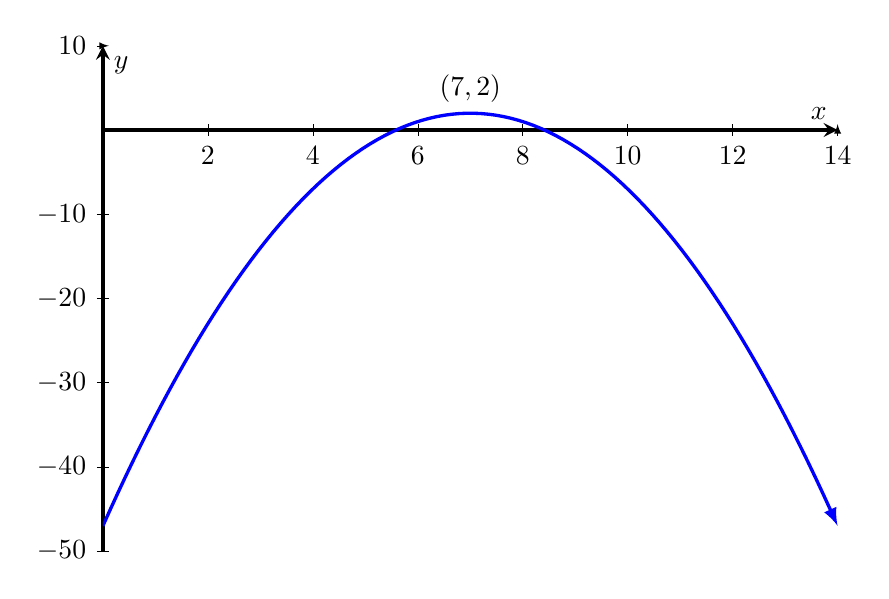
\begin{tikzpicture}
                \begin{axis}[
                    width=0.9\textwidth,
                    height=8cm,
                    axis lines = middle,
                    xlabel = $x$,
                    ylabel = $y$,
                    xmin=0, xmax=14,
                    ymin=-50, ymax=10,
                    tick style={black},
                    samples=100,
                    domain=0:14,
                ]
                
                    \addplot [blue, thick] {-(7-x)^2 + 2};
                    \node at (axis cs:7,2) [above] {\((7,2)\)};
                \end{axis}
            \end{tikzpicture}
            \caption{Wykres funkcji użytej do ewaluacji rozkładu godzin nauczycieli i klas na przestrzeni tygodnia.}
            \label{fig:funkcja_rownomiernosc}
        \end{figure}

        \subsubsection{Ocena względem nauczycieli}
            Ocena równomierności rozpoczyna się od obliczenia dla każdego nauczyciela wektora obciążenia godzinowego:
            \[ X_i = \begin{bmatrix} x_{i,1} & x_{i,2} & x_{i,3} & x_{i,4} & x_{i,5} \end{bmatrix} \]
            gdzie $x_{i,d}$ oznacza liczbę godzin lekcyjnych do przeprowadzenia przez $i$-tego nauczyciela $d$-tego dnia.
            
            Problemem funkcji kwadradowej jest fakt, że osobniki otrzymują dużą karę, kiedy zgodnie z przydziałem nauczyciel ma dzień wolny --- jest to niezgodne z założeniami.
            Wolimy, aby nauczyciej miał cztery dni 8-godzinne niż pięć dni po 6 lub 7 godzin.
            Aby osiągnąć taką właściwość zeruję wartość funkcji dla $x=0$, co skutkuje następującą funkcją:
            \[
                \begin{cases*}
                    f_T(x) = 0 & x = 0\\
                    f_T(x) = -\left(7-x\right)^2 + 2 & \text{ wpp.}\\
                \end{cases*}
            \]
            
            Następnie wyznaczam sumę wartości funkcji dla wszystkich argumentów tego wektora:
            \[ F_{c_{T_i}} = \sum_{d=1}^{5} f_T(x_{i,d}) \]
            gdzie $\left|\mathcal{T}\right|$ to liczba wszystkich nauczycieli.

            Końcowa ocena wszystkich nauczycieli to najzwyczajniej suma wszystkich wartości:
            \[ F_{c_T} = \sum_{i=1}^{\left|\mathcal{T}\right|} F_{c_{T_i}} \]

        \subsubsection{Ocena względem klas}
            Ocena równomierności godzin lekcyjnych dla klas jest analogiczna do poprzedniej.
            Tworzony jest wektor obciążenia godzinowego:
            \[ X_i = \begin{bmatrix} x_{i,1} & x_{i,2} & x_{i,3} & x_{i,4} & x_{i,5} \end{bmatrix} \]
            gdzie $g_{i,d}$ oznacza liczbę godzin lekcyjnych przez $i$-tej klasy $d$-tego dnia.

            W tym przypadku dni wolne nie są zgodne ze względu na ograniczenia opisane w~\ref{subsection:ograniczenia}, a więc modyfikacje funkcji nie są potrzebne.

            Analogicznie do nauczycieli tworzymy kolejno wektory i wartości:

            \noindent
            \begin{minipage}{.48\textwidth}
                \[ F_{c_{C_i}} = \sum_{d=1}^{5} f(x_{i,d}) \]
            \end{minipage}
            \begin{minipage}{.48\textwidth}
                \[ F_{c_C} = \sum_{i=1}^{\left|\mathcal{C}\right|} F_{c_{C_i}} \]
            \end{minipage}\\
            gdzie $\left|\mathcal{C}\right|$ to liczba wszystkich klas.

        \subsubsection{Normalizacja i wagi}
            Wyznaczanie końcowej wartości funkcji przystosowania wymaga uwzględnienia stosunku liczby nauczycieli do liczby uczniów.
            W typowych placówkach oświatowych liczba nauczycieli przywyższa liczbę klas.
            Bezpośrednie dodawanie ocen $F_{c_T} + F_{c_G}$ prowadziłoby do znaczącej dominacji oceny nauczycieli w ocenie końcowej.
            W celu rozwiązania tego problemu zastosowałem normalizację poprzez dzielenie każdej składowej przez odpowiednio $\left|\mathcal{T}\right|$ i $\left|\mathcal{C}\right|$.
            Takie podejście gwarantuje, że wpływ pojedynczej klasy na ocenę końcową jest porównywalny z wpływem pojedynczego nauczyciela.

            Kolejnym aspektem wymagającym uwzględnienia jest relatywna ważność obu kryteriów oceny. 
            W praktyce, wymagania równomiernego rozkładu dla każdej klasy są ważniejsze niż równomierny rozkład godzin nauczycieli.
            Aby umożliwić sterowanie tymi preferencjami należy zaimplementować wagi, co prowadzi do następującej postaci funkcji przystosowania:
            \[ F_c = \frac{\alpha_T}{\left|\mathcal{T}\right|} F_{c_T} + \frac{\alpha_G}{\left|\mathcal{C}\right|} F_{c_G}, \quad \alpha_T, \alpha_T \in \mathbb{R}^+ \]
            gdzie $\alpha_T$ to waga oceny nauczycieli, a $\alpha_G$ to waga oceny klas.

    \subsection{Selekcja}\label{subsection:selekcja}
        Zastosowałem traducyjną metodę ruletkową. Polega ona na losowaniu osobników, którzy posłużą jako rodzice z prawdopodobieństwami, które sa proporcjonalne do wartości ich funkcji przystowania.
        Mając wektor ocen $F_{c\text{ total}} = \begin{bmatrix} F_{c_1} & F_{c_1} & \cdots & F_{c_\mathfrak{P}} \end{bmatrix}$, gdzie $\mathfrak{P}$ to rozmiar populacji, sortujemy go i dzielimy go na pół.
        Drugą połowę populacji, która ma najgorsze wyniki, usuwam i na jej miejsce wstawiam potomków rodziców wylosowanych zgodnie z prawdopodobieństwami:
        \[ P = \begin{bmatrix} \sigma\left(F_{c_1}\right) & \sigma\left(F_{c_2}\right) & \cdots & \sigma\left(F_{c_\mathfrak{P}}\right) \end{bmatrix}, \quad \sigma(F_{c_i}) = \frac{\exp\left[F_{c_i}\right]}{\sum_{j=1}^{\mathfrak{P}} \exp\left[F_{c_j}\right] } \]
        W celu zamiany funkcji przystosowania na prawdopodobieństwa użyłem funkcji SoftMax.

    \subsection{Krzyżowanie}\label{subsection:krzyzowanie}
        Największym wyzwaniem podczas projektowania algorytmu okazało się opracowanie krzyżowania osobników, które zagwarantowałoby spójność z nałożonymi ograniczeniami.
        Niemożność zaimplementowania takich rozwiązań jak proste modyfikowanie krzyżowania jednopunktowego zmusiło mnie do opracowania specjalistycznych metod.

        Z uwagi na dwie składowe funkcji zdecydowałem się na zaimplementowanie dwóch niezależnych metod krzyżowania osobników.
        Takie podejście umożliwia równoczesne dziedziczenie cech związanych z optymalnym rozkładem zajęć zarówno z perspektywy nauczycieli, jak i klas.
        Pozwala to także na stworzenie dwóch różnych potomków z dwóch rodziców.

        \subsubsection{Względem oceny nauczycieli}
            Funkcja krzyżowania uwzględniająca ocenę rozkładu godzin nauczycieli definiuje się następująco:

            \noindent
            \textbf{Dane wejściowe:}
                \begin{itemize}
                    \item $S_1$ --- pierwszy rodzic
                    \item $S_2$ --- drugi rodzic
                    \item $F_{T_{S_1}}$ --- ocena nauczycieli pierwszego osobnika
                    \item $F_{T_{S_2}}$ --- ocena nauczycieli drugiego osobnika
                \end{itemize}
            
            \noindent
            \textbf{Proces:}
            \begin{enumerate}
                \item Inicjalizacja macierzy potomka: $S_{\text{child}} = \mathbf{0}_{5 \times \left|\mathcal{L}\right|}$
                \item Dla każdego nauczyciela $i \in \left\{1, 2, \dots, \left|\mathcal{T}\right|\right\}$:
                \begin{enumerate}
                    \item Jeżeli $F_{T_{i,S_1}} > F_{T_{i,S_2}}$, to dla każdego bloku $j$ prowadzonego przez nauczyciela $i$:
                    \begin{enumerate}
                        \item Przepisz kolumnę $j$ z macierzy $S_1$ do kolumny $j$ macierzy $S_{\text{child}}$
                    \end{enumerate}
                    \item W przeciwnym przypadku, dla każdego bloku $j$ prowadzonego przez nauczyciela $i$:
                    \begin{enumerate}
                        \item Przepisz kolumnę $j$ z macierzy $S_2$ do kolumny $j$ macierzy $S_{\text{child}}$
                    \end{enumerate}
                \end{enumerate}
            \end{enumerate}

            Wygenerowany w ten sposób osobnik $S_{\text{child}}$ ma cechy, które gwarantują jak najlepsze przypisanie nauczycieli wśród obu rodziców.
            Następną zaletą tego podejścia jest fakt, że gwarantuje to też także spełnienie wszystkich wymagań,
            jako że wszystkie wymagania odnoszą się do indywidualnych bloków, a tych nie zmieniamy, tylko przepisujemy.

        \subsubsection{Względem oceny klas}
            Analogicznie definiujemy krzyżowanie względem oceny klas:

            \noindent
            \textbf{Dane wejściowe:}
                \begin{itemize}
                    \item $S_1$ --- pierwszy rodzic
                    \item $S_2$ --- drugi rodzic
                    \item $F_{G_{S_1}}$ --- ocena klas pierwszego osobnika
                    \item $F_{G_{S_2}}$ --- ocena klas drugiego osobnika
                \end{itemize}
            
            \noindent
            \textbf{Proces:}
            \begin{enumerate}
                \item Inicjalizacja macierzy potomka: $S_{\text{child}} = \mathbf{0}_{5 \times \left|\mathcal{L}\right|}$
                \item Dla każdej klasy $i \in \left\{1, 2, \dots, \left|\mathcal{C}\right|\right\}$:
                \begin{enumerate}
                    \item Jeżeli $F_{G_{i,S_1}} > F_{G_{i,S_2}}$, to dla każdego bloku $j$ prowadzonego dla klasy $i$:
                    \begin{enumerate}
                        \item Przepisz kolumnę $j$ z macierzy $S_1$ do kolumny $j$ macierzy $S_{\text{child}}$
                    \end{enumerate}
                    \item W przeciwnym przypadku, dla każdego bloku $j$ prowadzonego przez nauczyciela $i$:
                    \begin{enumerate}
                        \item Przepisz kolumnę $j$ z macierzy $S_2$ do kolumny $j$ macierzy $S_{\text{child}}$
                    \end{enumerate}
                \end{enumerate}
            \end{enumerate}

            Wygenerowany w ten sposób osobnik $S_{\text{child}}$ ma cechy, które gwarantują jak najlepszy rozkład godzin lekcyjnych dla klas wśród obu rodziców.
            Podobnie w tym przypadku nie modyfikujemy przydziału godzin w indywidualnych blokach, więc zachowujemy zgodność z ograniczeniami.

    \subsection{Mutacja}\label{subsection:mutacja}
        Analogicznie do przypadku krzyżowania, zastosowanie prostych metod mutacji (takich jak losowa zamiana pojedynczych przydziałów) nie jest możliwe ze względu na wysokie ryzyko naruszenia ograniczeń.
        W szczególności, modyfikacja pojedynczych wartości macierzy $S$ może prowadzić do niezgodności z warunkiem głównym bloków.
        
        W odpowiedzi na to wyzwanie, przyjąłem strategię mutacji operującą na poziomie bloków --- kolumn macierzy przydziałów, podobną do podejścia zastosowanego w funkcji krzyżowania.
        Pozwana to na zachowania zgodności z ograniczeniami.
        
        \begin{samepage}
            Procedura mutacji definiuje się następująco:
            \begin{enumerate}
                \item Z populacji wybieranych jest losowo $n$ osobników.
                \item Dla każdego wybranego osobnika wybierany jest losowy podzbiór kolumn (bloków lekcyjnych).
                \item Dla każdej wybranej kolumny $j$ wylosuj nowy przydział zgodnie z procedurą opisaną w podrozdziale~\ref{subsection:generowanie_populacji}.
            \end{enumerate}
        \end{samepage}
        
        Takie podejście gwarantuje, że zmutowane osobniki zachowują zgodność z podstawowymi ograniczeniami problemu, jednocześnie wprowadzając do populacji nowe warianty rozkładów godzinowych wybranych bloków lekcyjnych.

        W celu zwiększenia stabilności procesu ewolucyjnego zaimplementowałem także elitarnego osobnika, który zawsze pojawia się niezmieniony w następnej generacji.
        Jest to osobik o największej wartości funkcji przystosowania:
        \[ S_{\text{best}} = S_i, \quad i = \underset{j \in \left\{1, 2, \dots \mathfrak{P}\right\}}{\arg\max} F_{c_j} \]

    \subsection{Przykładowe rezultaty}
        \textit{Przykładowe macierze z opisami}

\section{Solver programowania liniowego z ograniczeniami}\label{section:solver}
    W trzecim etapie algorytmu wykorzystuję solver programowania liniowego z ograniczeniami (Constraint Programming --- CP).
    W odróżnieniu od czystego programowania liniowego (MIP), solver CP operuje na szerszej klasie ograniczeń, w tym na zmiennych interwałowych, co czyni go idealnym narzędziem do problemów harmonogramowania.
    W odpowiedzi na wyzwania napotkane w podejściu opisanym w podrozdziale~\ref{subsection:podejscie_zerojedynkowe} zdecydowałem się na wykorzystanie zmiennych interwałowych opisanych dokładniej w dokumentacji OR-Tools~\cite{googleortoolsintervalvar}. 

    Zalety podejścia CP:
        \begin{itemize}
            \item \textbf{Naturalne modelowanie}: Zmienne interwałowe bezpośrednio reprezentują zajęcia o określonym czasie rozpoczęcia i zakończenia.
            \item \textbf{Efektywność pamięciowa}: W porównaniu z reprezentacją binarną z podrozdziału~\ref{subsection:podejscie_zerojedynkowe}, podejście interwałowe redukuje liczbę zmiennych decyzyjnych.
            \item \textbf{Specjalizowane ograniczenia}: Solver oferuje gotowe implementacje ograniczeń typowych dla harmonogramów --- nakładanie się interwałów.
        \end{itemize}

    Proces jest wykonywany niezależnie dla każdego dnia tygodnia $d \in \{1,2,3,4,5\}$, reprezentowanego przez wiersze macierzy $S_{\text{best}}$.
    Dla każdego dnia rozwiązujemy podproblem zawierający tylko te bloki $L_i$, dla których $S_{\text{best}_{d,i}}> 0$. \\
    Takie podejście:
    \begin{itemize}
        \item Redukuje wymagania pamięciowe o $\approx 5$.
        \item Umożliwia równoległe przetwarzanie dni, jeśli nie ogranicza nas pamięć.
        \item Upraszcza strukturę ograniczeń.
    \end{itemize}

    \subsection{Reprezentacja interwałów}
        Dla modelowania zajęć używamy zmiennych interwałowych, które reprezentują bloki czasowe o określonej długości:
        \begin{itemize}
            \item \textbf{Interwał podstawowy} dla bloku lekcyjnego $L_i \in \mathcal{L}$:
                \[
                    \begin{cases}
                        s_i &\in \left[0, H\right] \\
                        d_i &= v_i \\
                        e_i &\in \left[0, H\right] \\
                        e_i &= s_i + d_i    
                    \end{cases}
                \]
                gdzie $s_i$ to czas rozpoczęcia, $e_i$ to czas zakończenia, a $d_i$ to czas trwania.
            
            \item \textbf{Interwał opcjonalny} dla przypisania sali:
                \[
                    \begin{cases}
                        p_{i,j,r} &\in \left\{0, 1\right\}\\
                        p_{i,j,r} &\implies e_i = s_i + d_i
                    \end{cases}
                \]
        \end{itemize}

    \subsection{Zmienne decyzyjne}
        \subsubsection{Interwały bloków lekcyjnych}
            Dla każdego bloku $L_i \in \mathcal{L}$ z liczbą godzin $v_i > 0$ definiujemy:
            \[ I_i = (s_i, v_i, e_i) \]

        \subsubsection{Przypisania sal}
            Dla każdej możliwej kombinacji (blok, nauczyciel, sala) definiujemy interwał opcjonalny:
            \[ O_{L_i,t,r} = (s_i, v_i, e_i, p_{L_i,t,r}), \quad \begin{cases}
                L_i &\in \mathcal{L} \\
                t &\in \mathcal{T} \\
                r &\in \mathcal{R}
            \end{cases} \]
            gdzie brane pod uwagę są tylko mozliwe kombinacje. Przykładowo blok lekcyjny z jednym wymaganiem głównym matematyki, nauczyciel matematyki oraz sala do matematyki.

    \subsection{Ograniczenia}
        \subsubsection{Ograniczenie przypisania sal}
            Dla każdego bloku $L_i$ musi być przypisana odpowiednia liczba sal:
            \[ \forall L_i \in \mathcal{L}: \sum_{r \in \mathcal{R}, t \in \mathcal{T}} p_{L_i,t,r} = |T_i| \]

        \subsubsection{Ciągłość zajęć dla klas}
            Dla każdej klasy $c \in \mathcal{C}$ i dnia $d \in \{1, 2, \dots,5\}$:
            \[ \mathcal{L}_{c,d} = \{L_i \in \mathcal{L}: \exists w \in L_i \text{ takie, że } c_w = c \land s_{\text{best}_{d,i}} > 0\} \]
            \textbf{Nienakładanie się zajęć}~\cite{googleortoolsoverlap}\textbf{:}
            \[ \text{AddNoOverlap}(\{I_i : L_i \in \mathcal{L}_{c,d}\}) \]
            \textbf{Brak okienek:}
            \[
                \begin{cases}
                    \text{start}_c = \min\{s_i : L_i \in \mathcal{L}_{c,d}\} \\
                    \text{end}_c = \max\{e_i : L_i \in \mathcal{L}_{c,d}\} \\
                    \text{end}_c - \text{start}_c = \sum_{L_i \in \mathcal{L}_{c,d}} v_i
                \end{cases}
            \]

        \subsubsection{Nakładanie się nauczycieli}
            Dla każdego nauczyciela $t \in \mathcal{T}$ i dnia $d \in \{1, 2, \dots,5\}$:
            \[ \mathcal{L}_{t,d} = \{L_i \in \mathcal{L}: t \in T_i \land s_{\text{best}_{d,i}} > 0\} \]
            \[ \text{AddNoOverlap}(\{I_i : L_i \in \mathcal{L}_{t,d}\}) \]

        \subsubsection{Kolizje sal}
            Dla każdej sali $r \in \mathcal{R}$ i dnia $d \in \{1, 2, \dots,5\}$:
            \[ \mathcal{O}_{r,d} = \{O_{L_i,t,r} : L_i \in \mathcal{L}, t \in \mathcal{T}, s_{\text{best}_{d,i}} > 0\} \]
            \[ \text{AddNoOverlap}(\mathcal{O}_{r,d}) \]
        
        \subsubsection{Sekwencjonowanie przedmiotów}
            Ograniczenie dotyczące dwuch takich samych przedmiotów jednego dnia jest łatwo rozwiązywane poprzez zastosowanie interwałów, gdyż z definicji mamy zagwarantowane, że:
            \[ \forall i \in \left\{1, 2, \dots, \left|\mathcal{L}\right|\right\}: v_i = 2 \implies e_i - s_i = 2 \]
            W ten sposób jeśli do danego dnia są przypisane dwie godziny $i$-tego bloku, to mamy gwarancję, że następują one po sobie.

    \subsection{Funkcja celu}
        Minimalizujemy całkowity czas przebywania nauczycieli w szkole:
        \[
            \forall t \in \mathcal{T}, d \in \{1,2,\dots,5\}:
            \begin{cases}
                \text{start}_{t,d} &= \min\{s_i : L_i \in \mathcal{L}_{t,d}\} \\
                \text{end}_{t,d} &= \max\{e_i : L_i \in \mathcal{L}_{t,d}\} \\
                \text{duration}_{t,d} &= \text{end}_{t,d} - \text{start}_{t,d}
            \end{cases}
        \]

        \[ F_c = \sum_{t \in \mathcal{T}} \sum_{d=1}^{5} \text{duration}_{t,d} \]

        Minimalizacja tej funkcji prowadzi do kompaktowego układania zajęć, redukując okienka w planach nauczycieli.

    \subsection{Transformacja interwałów na przypisania końcowe}
        Po znalezieniu rozwiązania przez solver CP-SAT, konieczne jest przekształcenie zmiennych interwałowych na ostateczne przypisania w zbiorze $\mathcal{Z}$.
        Proces ten obejmuje ekstrakcję wartości zmiennych decyzyjnych i mapowanie na strukturę danych planu lekcji.
        
        \subsubsection{Ekstrakcja rozwiązań z solvera}
            Dla każdego interwału $I_i$ w rozwiązaniu zapisujemy następujące wartości:
            \begin{itemize}
                \item $L_i$
                \item $s_i$
                \item $e_i$
                \item $v_i$
                \item $d$ --- aktualnie przetwarzany dzień tygodnia
                \item $\mathcal{R}_i = \left\{r \in \mathcal{R}: \exists t \in \mathcal{T} \text{ takie, że } p_{i,t,r} = 1 \right\}$ --- zbiór aktywnych sal, które zostały przypisane do bloku $L_i$.
            \end{itemize}
        
        \subsubsection{Mapowanie na strukturę lekcji}
            Dla każdych takich wartości tworzymy konkretne lekcje w zbiorze $\mathcal{Z}$.
            Wpierw tworzymy funkcję, która będzie przypisywać nauczycieli i prowadzone przez nich przedmioty $s$ do odpowiednich sal.
            \begin{align*}
                f: T_i &\to \mathcal{R}_i \\
                \forall t \in T_i: f(t) &= r \in \mathcal{R}_i \text{ takie, że } r \text{ obsługuje przedmiot } s \in \vec{S}_{L_i}
            \end{align*}
            Konieczne jest użycie takiej funkcji, ponieważ każdy nauczyciel w jednym bloku może mieć przypisane wiele klas.
            Musimy stworzyć wiele przypisań, które będą miały taką samą salę $r$ dla każdej klasy.

            Dla każdego wymagania $w \in L_i$ i każdego slotu czasowego $h \in \left[1, e_i-s_i\right]$:
            \begin{align*}
                z &= (d, h, c_w, t_w, s_w, f(t_w)) \\
                \mathcal{Z}_d &\gets \mathcal{Z}_d \cup \{z\}
            \end{align*}
        
        \subsubsection{Przykład transformacji}
            Rozważmy blok $L_i = \{w_1, w_2\}$ z $v_i = 2$, gdzie:
            \begin{itemize}
                \item $w_1 = (t_1, c_1, s_1, 3)$ --- nauczyciel $t_1$, klasa $c_1$, wychowanie fizyczne
                \item $w_2 = (t_2, c_1, s_2, 3)$ --- nauczyciel $t_2$, klasa $c_1$, wychowanie fizyczne
            \end{itemize}
            
            Po rozwiązaniu otrzymujemy przypisania:
            \begin{align*}
                z_1 &= (1, 2, c_A, t_1, s_1, r_1) \\
                z_2 &= (1, 3, c_A, t_1, s_1, r_1) \\
                z_3 &= (1, 2, c_A, t_2, s_2, r_2) \\
                z_4 &= (1, 3, c_A, t_2, s_2, r_2)
            \end{align*}

            Jest to równoznaczne z leckją wychowania fizycznego podzieloną na dwie grupy, które odbywają się w tym samym czasie.
        
        Proces ten powtarzamy dla wszystkich dni tygodnia, tworząc kompletny plan lekcji $\mathcal{Z} = \bigcup_{d=1}^5 \mathcal{Z}_d$ spełniający wszystkie ograniczenia i optymalizujący funkcję celu.

\section{Wyniki}
    \begin{itemize}
        \item Dlaczego moje wyniki są wspaniałe
        \item Średni czas potrzebny na generację planu
    \end{itemize}

    \subsection{Statystyki planu}
        \begin{itemize}
            \item Ilość okienek
            \item Rozkład lekcji w tygodniu
            \item Lekcje początkujące/kończące
            \item Statystyki nauczycieli, godziny w szkole do godzin lekcyjnych (płatnych)
        \end{itemize}

    \subsection{Porównanie z ręcznie ułożonym planem}
        Porównanie z planem, który szkoła ułożyła ręcznie.